%
% This is the LaTeX template file for lecture notes for EE 382C/EE 361C.
% This template is based on the template for Prof. Sinclair's CS 270.

\documentclass[twoside]{article}
\usepackage{graphics}
\usepackage{tikz}
\setlength{\oddsidemargin}{0.25 in}
\setlength{\evensidemargin}{-0.25 in}
\setlength{\topmargin}{-0.6 in}
\setlength{\textwidth}{6.5 in}
\setlength{\textheight}{8.5 in}
\setlength{\headsep}{0.75 in}
\setlength{\parindent}{0 in}
\setlength{\parskip}{0.1 in}

%
% The following commands set up the lecnum (lecture number)
% counter and make various numbering schemes work relative
% to the lecture number.
%
\newcounter{lecnum}
\renewcommand{\thepage}{\thelecnum-\arabic{page}}
\renewcommand{\thesection}{\thelecnum.\arabic{section}}
\renewcommand{\theequation}{\thelecnum.\arabic{equation}}
\renewcommand{\thefigure}{\thelecnum.\arabic{figure}}
\renewcommand{\thetable}{\thelecnum.\arabic{table}}

%
% The following macro is used to generate the header.
%
\newcommand{\lecture}[4]{
   \pagestyle{myheadings}
   \thispagestyle{plain}
   \newpage
   \setcounter{lecnum}{#1}
   \setcounter{page}{1}
   \noindent
   \begin{center}
   \framebox{
      \vbox{\vspace{2mm}
    \hbox to 6.28in { {\bf EE 382V Social Computing
                        \hfill Fall 2018} }
       \vspace{4mm}
       \hbox to 6.28in { {\Large \hfill Lecture #1: #2  \hfill} }
       \vspace{2mm}
       \hbox to 6.28in { {\it Lecturer: #3 \hfill Scribe: #4} }
      \vspace{2mm}}
   }
   \end{center}
   \markboth{Lecture #1: #2}{Lecture #1: #2}
   %{\bf Disclaimer}: {\it These notes have not been subjected to the
   %usual scrutiny reserved for formal publications.  They may be distributed
   %outside this class only with the permission of the Instructor.}
   \vspace*{4mm}
}

%
% Convention for citations is authors' initials followed by the year.
% For example, to cite a paper by Leighton and Maggs you would type
% \cite{LM89}, and to cite a paper by Strassen you would type \cite{S69}.
% (To avoid bibliography problems, for now we redefine the \cite command.)
% Also commands that create a suitable format for the reference list.
\renewcommand{\cite}[1]{[#1]}
\def\beginrefs{\begin{list}%
        {[\arabic{equation}]}{\usecounter{equation}
         \setlength{\leftmargin}{2.0truecm}\setlength{\labelsep}{0.4truecm}%
         \setlength{\labelwidth}{1.6truecm}}}
\def\endrefs{\end{list}}
\def\bibentry#1{\item[\hbox{[#1]}]}

%Use this command for a figure; it puts a figure in wherever you want it.
%usage: \fig{NUMBER}{SPACE-IN-INCHES}{CAPTION}
\newcommand{\fig}[3]{
			\vspace{#2}
			\begin{center}
			Figure \thelecnum.#1:~#3
			\end{center}
	}
% Use these for theorems, lemmas, proofs, etc.
\newtheorem{theorem}{Theorem}[lecnum]
\newtheorem{lemma}[theorem]{Lemma}
\newtheorem{proposition}[theorem]{Proposition}
\newtheorem{claim}[theorem]{Claim}
\newtheorem{corollary}[theorem]{Corollary}
\newtheorem{definition}[theorem]{Definition}
\newenvironment{proof}{{\bf Proof:}}{\hfill\rule{2mm}{2mm}}

% **** IF YOU WANT TO DEFINE ADDITIONAL MACROS FOR YOURSELF, PUT THEM HERE:

\begin{document}
%FILL IN THE RIGHT INFO.
%\lecture{**LECTURE-NUMBER**}{**DATE**}{**LECTURER**}{**SCRIBE**}
\lecture{21}{October 27}{Vijay Garg}{Robert Pate}
%\footnotetext{These notes are partially based on those of Nigel Mansell.}

% **** YOUR NOTES GO HERE:

% Some general latex examples and examples making use of the
% macros follow.  
%**** IN GENERAL, BE BRIEF. LONG SCRIBE NOTES, NO MATTER HOW WELL WRITTEN,
%**** ARE NEVER READ BY ANYBODY.
\section{Background on Lattice Linear Predicates}

We proved some things about stable marriage, such as stable matching always exists, but with Lattice Linear Predicates we can prove it more easily and apply the same approach to the biggest problems such as housing allocation, market clearing, etc. 

We had algorithms already for all of these problems but this gives us extra insight into them. 

\section{Consistent Global State}
\begin{definition}
Lattice

A poset where a join and meet exist for all pairs of elements
\end{definition}

\begin{definition}
Distributive Lattice

Lattice where joins and meets distribute over each other. 
\end{definition}

For example we have an example poset below where there are 4 elements, the events are proposals, and the orderings indicate the order the proposals were done.

\begin{tikzpicture}
\draw [->] (0,0) -- (1,0);
\draw [->] (0,1) -- (1,.2);
\draw [->] (0,1) -- (1,1);
\draw[fill] (-.2,0) circle [radius=2pt] node [left] {$f_1$};
\draw[fill] (-.2,1) circle [radius=2pt] node [left] {$e_1$};
\draw[fill] (1.2,1) circle [radius=2pt] node [right] {$e_2$};
\draw[fill] (1.2,0) circle [radius=2pt] node [right] {$f_2$};
\end{tikzpicture}

From this poset we define a 2nd poset $X (e_1, e_2, f_1, f_2)$ which has the same 4 elements. There are 16 possible subsets, but we don't want all of them. We want just the "consistent global states." This is also used in distributive systems by treating this as the order of events in a system.

\begin{definition}
Consistent Global State

$G$, a subset of $X$, is a CGS if\\
$\forall$ $e, f \in X$ : ($f \in G) \land (e < f) \Rightarrow e \in G$

\end{definition}

\textbf{Graph of X drawn upward:}

\begin{tikzpicture}
\filldraw 
(0,0) circle (2pt) node[align=center, below] {\{ \} \\ empty set} --
(-1,1) circle (2pt) node[align=right, left] {\\$e_1$\\ meet always intersection} --
(-2,2) circle (2pt) node[align=left, left] {$e_1, e_2$} --
(-1,3) circle (2pt) node[align=left, left] {$e_1, e_2, f_1$} --
(0,4) circle (2pt) node[align=center, above] {$e_1, e_2, f_1, f_2$}

(0,0) --
(1,1) circle (2pt) node[align=right, right] {$f_1$}

(2,2) circle (2pt) node[align=left, right] {$f_1, f_2$\\ not CGS, includes $f_2$ but not $e_1$ which proceeds $f_2$}

(1,1) -- 
(0,2) circle (2pt) node[align=left, left] {$e_1, f_1$} --
(-1,3)

(-1,1) -- (0,2) -- 
(1,3) circle (2pt) node[align=right, right] {$e_1, f_1, f_2$} --
(0,4)

;
\end{tikzpicture}

We started with the smallest at the bottom which is always the empty set, and draw each of the consistent global states. This also draws a natural ordering relationship between them because our $<$ relation is defined by being a subset of.

\begin{claim}
A set of CGS is a distributive lattice

\begin{proof}
Definitions:\\
Elements: all are CGS due to our claim\\
Lattice: our relation must be poset ("subset of" is reflexive, anti-symmetric, and transitive)\\
Distributive: must be closed under meets and joins (a meet of multiple CGS is an intersection of them)

So we must show:\\
$G$ is a CGS $\land$ $H$ is a CGS  $\Rightarrow$ $G \cap H$ is a CGS

Meet is greatest lower bound. $G \cap H$ is lower than $G$ because any intersection is smaller. It's also the greatest lower bound because we can have elements lower than $G \cap H$.

1. Pick any two events where:\\
\verb'  '$e,f \in X$\\
\verb'  '$f \in G \cap H$\\
\verb'  '$e < f$\\
Now we prove $e \in G \cap H$:

2. $f \in G \cap H$ implies $(f \in G) \land (f \in H)$.

3. $(e < f) \land (G$ is CGS) $\Rightarrow e \in G$.

4. $(f \in H) \land (e < f) \Rightarrow e \in H$

5. $(e \in H) \land (e \in G) \Rightarrow e \in G \cap H$

\end{proof}

\end{claim}

\subsection{Drawing a poset on a time line}

\begin{tikzpicture}
\draw [->] (1,1) -- (2,1) node [right] {Time};
\draw [dashed] (0,-.5) node [align=right, below] {Intersection on this side\\} -- (3,-.5) ;
\draw [-] (0,0) -- (5,0);
\draw [-] (0,-1) -- (5,-1);
\draw [-] (0,-2) -- (5,-2);
\draw [->] (3,.5) -- (5.5,-2.5) node [left] {$H$};
\draw [->] (3.5,-2.5) -- (5, 1) node [left] {$G$};
\draw [red, <-] (2, -2) -- (5, -1) node [right] {$e$, this should never happen!};
\draw[red, fill] (2,-2) node[align=center, below] {$f$};
\end{tikzpicture}

There cannot be arrows going backwards (such as $e, f$ as pictured above) in a CGS since it would no longer be consistent. Consistent means for every included event, all prior events are also included. In the above picture, $e$ proceeds $f$, but $e$ isn't in $G$ nor $H$ therefore they could not be consistent global states.

\subsection{Unions}
We've shown this works for meets, a similar argument can be made to show it's also  closed under joins where the relation is unions instead of intersections.

\section{Lattice Linear Predicates}

Back to our example, these events could be proposals from men to women or proposals from buyers to sellers.  And the subsets tells us what has happened so far and tells us the state of the system.

It depends on the problem you're looking at, but in the example of the Stable Matching Problem, a state is "good" if the current state of proposals forms a stable matching. 

Our goal would be to find the states that are good for us. We'll define a boolean predicate that's much easier to analyze called a Lattice Linear Predicate.

\begin{definition}
Lattice Linear Predicate

Given a distributive lattice $L$ and given a boolean predicate $B$, $B$ is a Lattice Linear Predicate if:\\
$\forall$ CGSs $G$: $\neg B(G) \Rightarrow \exists$ $i$:forbidden$(G, i, B)$
\end{definition}

\textbf{LLP Example}

If you're happy, you're done.

If not, there must be some process, such as a man in SMP, that if it doesn't move then you cannot reach a good state (such as a stable marriage). If we can find him, then we can advance him to proceed toward stable marriage.

Back to the lattice, start with the lowest set (always empty set) then proceed to $e_1$ or $f_1$. The problem is that the lattice could be huge! If some predicate is LLP it saves us from having to explore the entire lattice. It lets us know a given combination is bad so we can throw it away and continue. Any point that we find is forbidden we know all older points are also forbidden since we're dealing with Consistent Global States. For the same reason, and any future states where we haven't advanced the problem process are also forbidden.


\begin{definition}
Berkoff's Theorem

In any CGS, if my predicate is not true, unless I advance, it can never be true.
\end{definition}

\begin{definition}
Forbidden

Given any distributive lattice $L$ and predicate $B$ \\
forbidden $(G, i, B) \equiv$ \\
$\forall H \in L$ : $G \leq H$ : \\
$(G[i] = H[i])$ $\Rightarrow \neg B(H)$

\end{definition}

\begin{tikzpicture}
\draw [-] (0,0) -- (5,0);
\draw [-] (0,-1) node [left] {process $P_i$} -- (5,-1);
\draw [-] (0,-2) -- (5,-2);
\draw [-] (2,-1) -- (5.5,.5) node [left] {$H$};
\draw [-] (2,-1) -- (5.5,-2.5);
\draw [-] (2,.5) node [left] {One set of proposals that didn't work, $G$} -- (2, -2.5);
\draw[fill] (2,-1) circle (2pt);
\draw [->, dashed] (0, -3) node[align=left, below] {a proposal resulting\\in unstable match $G$} -- (1.8, -1.1);
\end{tikzpicture}

Consider the point pictured above. Think of it as a proposal that results in an unstable matching $G$. There are at least one of these such that if we continue around it we'll never succeed. In any state in the future from here (such as $H$) it will not be good because of this blocking pair. 

This is valuable in helping us prune our search space to speed up our algorithms, if we can find it.

\textbf{Simple Example Forbidden Process:}

\begin{tikzpicture}
\draw [->] (0,0) -- (1,0);
\draw [->] (0,1) -- (1,.2);
\draw [->] (0,1) -- (1,1);
\draw[fill] (0,0) node [left] {$f_1$};
\draw[fill] (-.5,0) node [left] {$p_2$};
\draw[fill] (0,1) node [left] {$e_1$};
\draw[fill] (-.5,1) node [left] {$p_1$};
\draw[fill] (1,1) node [right] {$e_2$};
\draw[fill] (1,0) node [right] {$f_2$};
\end{tikzpicture}

Given a predicate $B(G) \equiv$ "any state which contains at least one event from $p_2$." Unless we execute one event from $p_2$, we'll never make the predicate true. So $p_2$ is the forbidden process, and $\{ \}, \{e_1\}, \{e_1, e_2\}$ are all bad states.

\begin{claim}
$B$ is a lattice linear if and only if $B$ is "closed under meets."\\
$B$ is true in $G$ $\land$ $B$ is true in $H$ $\Rightarrow B(G \cap H)$.

If true in 2 places, find meet. If false then not lattice linear. So if not true in $e_1$, should be at least 1 dimension that if I don't progress on it I can never make it true. So if I can advance something else to make $B$ true then $e_1$ is not forbidden.

\end{claim}


\section{Lattice Linear Algorithm}

\subsection{Recap}
\begin{enumerate}
\item Defined notion of predicate on a lattice
\item Defined which predicates are good
\item Defined closure of meets
\end{enumerate}
Some predicates are nice from both meet and join perspectives, such as SMP, but not all. 
Payoff: if algorithm is lattice linear then it's efficient

\subsection{LLP Algorithm to find the minimum feasible vector}

\begin{itemize}
    \item One variable: where are you in the lattice, as a global vector $G$
    \item init $G$ as the least CGS in the lattice
    \item return $G$ as the least CGS that is feasible, e.g. minimum market clearing price
    \item $B$ feasible predicate: an assignment is feasible if for example it's a stable marriage or market clearing price
    \item Set an upper bound $T$ that is the top most element, such as the number of women. Top is the end, bottom is the start.
    \item Note this is a generic algorithm, but "forbidden" will differ for each type of problem
    \item "Successor" is defined in respect to chain in poset. Go to next event on the same process. 
    \item Never define the whole lattice, it's huge. break poset into chains (however you want) and call them processes, so long as lattice linear.
    \item Max time: total count of events $O(n^2)$
\end{itemize}

\texttt{
vector function getLeastFeasible ($T$: vector, $B$: predicate)\\
$~~~~$var $G$: the least CGS in the lattice \\
$~~~~$while ($\exists$ $j$ : forbidden $(G, j, B)$ do\\
$~~~~ ~~~~$ for all $j$ in forbidden$(G, j, B)$:\\
$~~~~ ~~~~ ~~~~$ if $(G[j] = T[j])$ then return null // reached the top, no feasible vector \\
$~~~~ ~~~~ ~~~~$ else $G[j] := $ successor of $G_j$\\
end while\\
return $G$
}

$\forall j$ : forbidden $(G, j, B)$ is equivalent to $\neg B(G)$ because $B$ is lattice linear. If this is not true it implies there must exist something that is forbidden. So if your predicate is not true, find one that is forbidden and advance that.

\section{Proving lattice-linearity of predicates}

\begin{lemma}
Lattice Linearity has the property:\\
if $B_1$ is $LL$ $\land$ $B_2$ is $LL$ $\Rightarrow$ $B_1 \land B_2$ is $LL$
\end{lemma}

\begin{proof}
\begin{enumerate}
    \item Pick any global state and if it's not true here, we can find a forbidden
    \item Find the forbidden: if $B_1 \land B_2$ is not true, then either $B_1$ is not true or $B_2$ is not true.
    \item Say $B_1$ is not true, and we know $B_1$ is LL then there exists at least one place we can advance to make it true
    
    \item You'll find at least one process on which you must advance
\end{enumerate}

\end{proof}

\section{Conclusion}

Goal for next session is be able to show:
\begin{itemize}
\item SMP predicate is lattice linear
\item Market clearing price is lattice linear
\item Housing allocation problem is lattice linear
\item And that the same algorithm works for all 3
\end{itemize}





\end{document}





